\section{Introduction}
\begin{frame}
\frametitle{Machine Learning (Recap)}
\begin{itemize}
	\visible<1->{\item{What is machine learning?}}
	
\end{itemize}
\begin{figure}[h]
	\begin{tikzpicture}[scale=1]
	\visible<2->{\pgftext{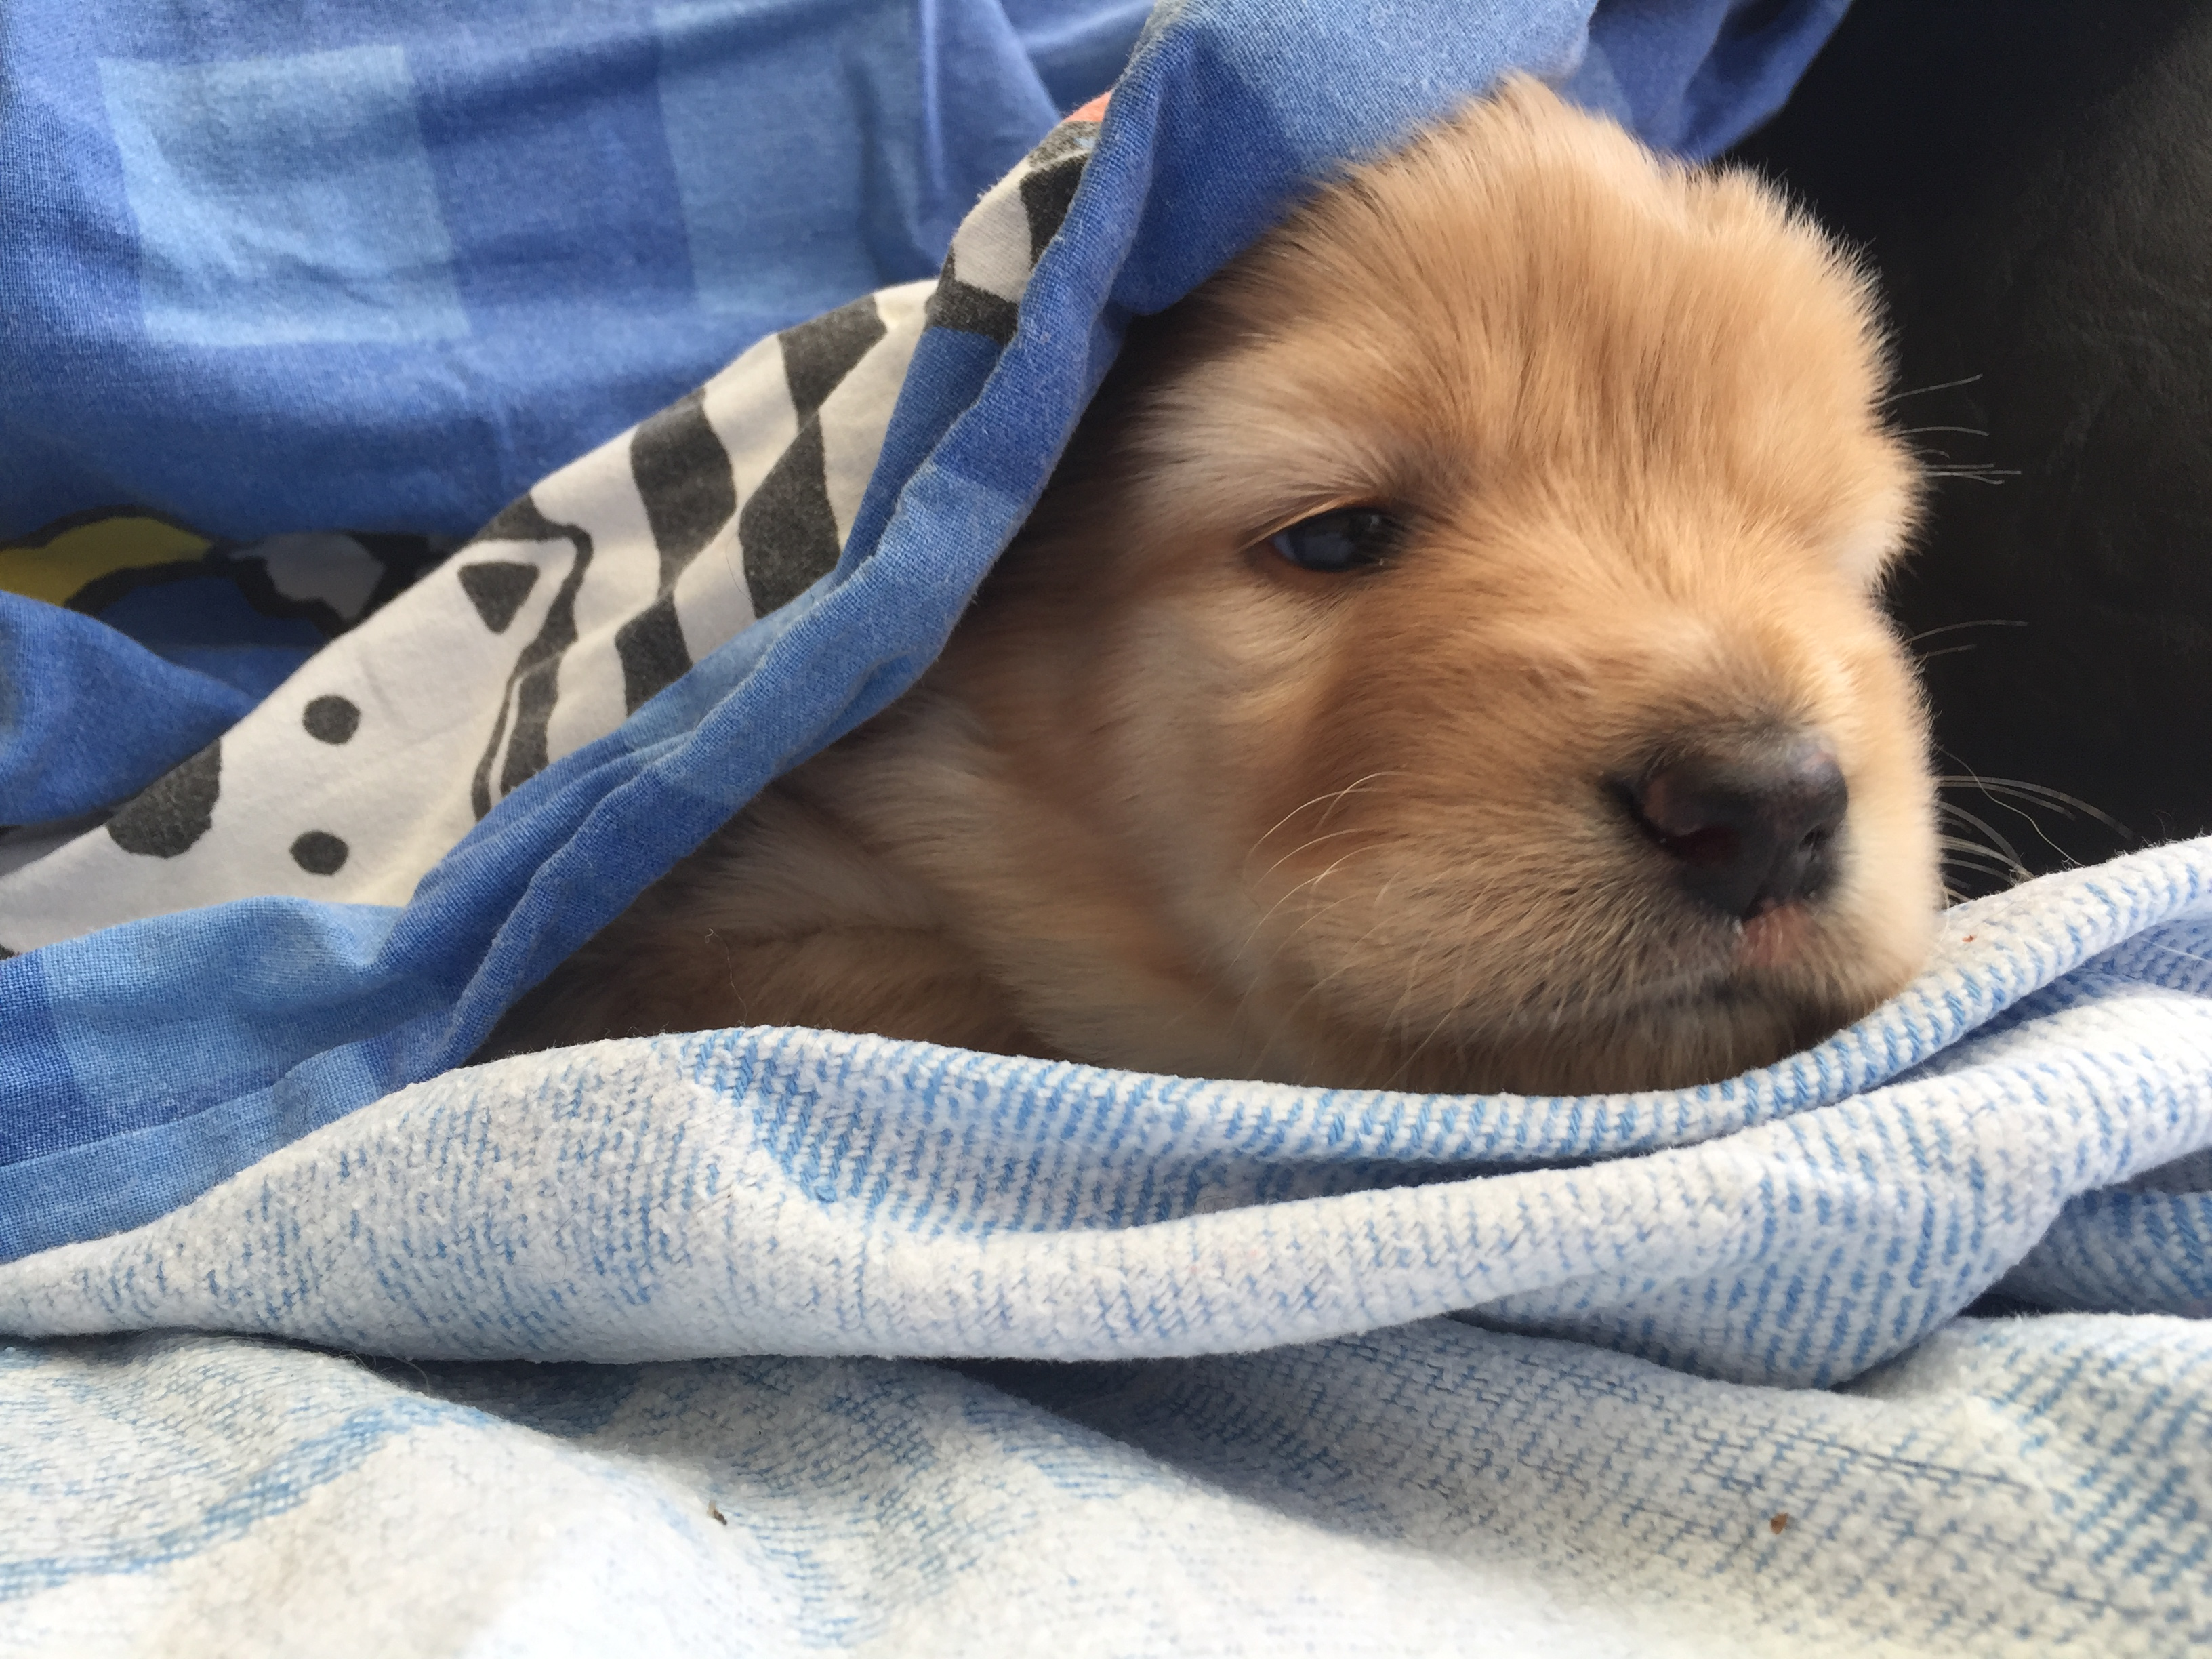
\includegraphics[width=150pt]{./figs/dog.jpg}} at (0, 0);
	\coordinate (x1) at (2.5, 0);
	}
	\visible<3->{
		\draw[->] (x1) -- (5, 0);
	}
	\visible<4->{
		\draw[->, fill=black] (5,-1) rectangle (7, 1);
		\draw[white] (6, 0) node{$f$};
	}
	\visible<3->{\draw[->] (7, 0) -- (9, 0) node[right]{dog};}
	\end{tikzpicture}
\end{figure}

\begin{itemize}
	\visible<5->{\item{By knowing a set of data and their targets we can tune f to output what we want.}}
	
\end{itemize}
\end{frame}
\begin{frame}
\frametitle{Machine Learning (Recap)}
\begin{itemize}
	\visible<2->{\item{We don't have to define endless rules}}
	\visible<3->{\item{It can write computational rules nobody of us would ever think of}}
	\visible<4->{\item{It can often write better computational rules than we could}}
	\visible<5->{\item{It can check more cases than we could}}
\end{itemize}
\end{frame}

\begin{frame}
\frametitle{Validating Machine Learning (Recap)}
\begin{figure}[h]
	\centering
	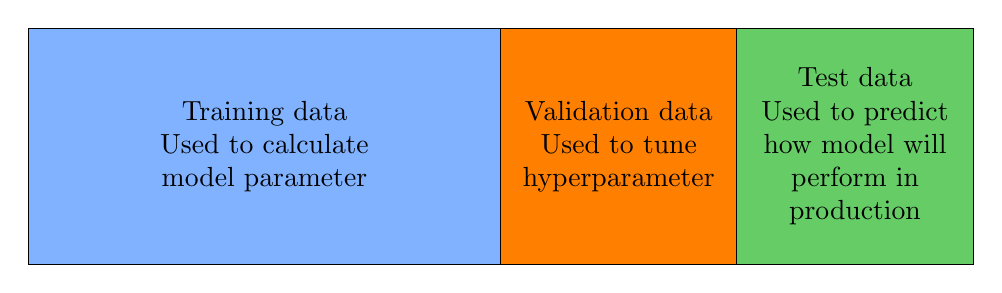
\begin{tikzpicture}
	
	\definecolor{lightblue}{rgb}{0.5,0.7,1}
	%\definecolor{lightred}{rgb}{1,.6,.6}
	\definecolor{lightred}{rgb}{1,.6,.3}
	\definecolor{lightgreen}{rgb}{.4,.8,.4}
	\definecolor{lightpurple}{rgb}{.8,.4,.8}
	\definecolor{lightgrey}{rgb}{.8,.8,.8}
	
	% 4th Column
	\visible<2->{\draw[fill=lightblue] (0,0) rectangle (6,3) (3,1.5) node[align=center]{Training data \\Used to calculate\\model parameter};}
	\visible<3->{\draw[fill=orange] (6,0) rectangle (9,3) (7.5,1.5) node[align=center]{Validation data \\Used to tune\\hyperparameter};}
	\visible<4->{\draw[fill=lightgreen] (9,0) rectangle (12,3) (10.5,1.5) node[align=center]{Test data \\Used to predict\\how model will\\perform in\\production};}
	
	\end{tikzpicture}
\end{figure}
\end{frame}

\section{Overview}

\begin{frame}
\frametitle{Today's Overview}
\begin{itemize}
	\visible<2->{\item 9:00 Introduction to Deep Learning
		\begin{itemize}
			\item Short recap on machine learning
			\item Build and train a perceptron in numpy
			\item Change the code to use PyTorch
			\item Gradient Descent
		\end{itemize}	
	}	
	\visible<3->{\item 10:30 Coffee Break}
	\visible<4->{\item 10:45 Neural Networks
		\begin{itemize}
			\item Implement a multi-layer perceptron
			\item Recurrent neural networks
		\end{itemize}
	}
	\visible<5->{\item 12:00 Lunch}
	\visible<6->{\item 13:00 RNN (continued)}
	\visible<7->{\item 13:30 Word2Vec}
	\visible<8->{\item 14:30 Coffee Break}
	\visible<9->{\item 14:45 Chatbot}
	\visible<10->{\item 16:00 End of workshop}
\end{itemize}
\end{frame}

\section{Perceptron}
\begin{frame}
\frametitle{Perceptron}
\begin{minipage}{.4\textwidth}
	\begin{itemize}
		\visible<1->{\item The perceptron contains a weight ($\vec{w}$) for each input and a threshold ($\Theta$)}
		\visible<3->{\item Its output can be calculated as $\sum\limits_{i=0}^{k} w_i X_i \geq \Theta$}
	\end{itemize}
\end{minipage}
\begin{minipage}{.55\textwidth}
\begin{figure}[h]
	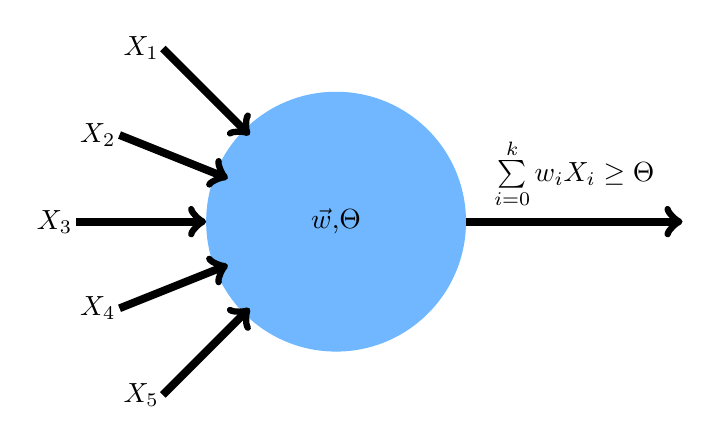
\begin{tikzpicture}[scale=.55]
		\definecolor{lightblue}{rgb}{.2,.6,1}
		\definecolor{lightred}{rgb}{.8,.2,.2}
		\definecolor{lila}{rgb}{.6,.2,.6}
		\visible<1->{\coordinate (Unit) at (0,0);
			\fill[fill=lightblue, opacity = .7] (Unit) circle(3);
			\draw (Unit) node{$\vec{w}$,$\Theta$};}
		\visible<2->{
			\coordinate (x1) at (-4,4);
			\draw (x1) ++(-.5,0) node{$X_1$};
			\coordinate (x2) at (-5,2);
			\draw (x2) ++(-.5,0) node{$X_2$};
			\coordinate (x3) at (-6,0);
			\draw (x3) ++(-.5,0) node{$X_3$};
			\coordinate (x4) at (-5,-2);
			\draw (x4) ++(-.5,0) node{$X_4$};
			\coordinate (x5) at (-4,-4);
			\draw (x5) ++(-.5,0) node{$X_5$};
		}
		\visible<2->{
			\draw[->, line width=1mm] (x1) -- (-2,2);
			\draw[->, line width=1mm] (x2) -- (-2.5,1);
			\draw[->, line width=1mm] (x3) -- (-3,0);
			\draw[->, line width=1mm] (x4) -- (-2.5,-1);
			\draw[->, line width=1mm] (x5) -- (-2,-2);
		}
		\visible<3->{
			\draw[->, line width=1mm, decorate] (3,0) -- node[above]{$\sum\limits_{i=0}^{k} w_i X_i \geq \Theta$} (8,0) ;
		}
	\end{tikzpicture}
\end{figure}
\end{minipage}
\end{frame}

\begin{frame}
\frametitle{Perceptron Training}
\begin{itemize}
	\visible<2->{\item Start with random weights}
	\visible<3->{\item{Calculate the perceptron's estimate of the solution with: $\hat{y} = \left(\sum\limits_{i} w_i X_i \geq 0\right)$}}
	\visible<4->{\item{Determine the update for the weights using the error and the learning rate ($\alpha$): $\partial w_i = \alpha (y-\hat{y}) X_i$}}
	\visible<5->{\item{Calculate new weights as: $w_i \leftarrow w_i + \partial w_i$}}
	\visible<6->{\item Restart the process until the solution is found}
	\visible<7->{\item Let us actually implement this in the first notebook (Perceptron)}
\end{itemize}
\end{frame}

\begin{frame}
\frametitle{Conclusions}
\begin{itemize}
	\visible<2->{\item Congratulations on training your first perceptron! You just taught a computer to learn!}
	\visible<3->{\item Why didn't we wait for the final weights, but stop after one run over the dataset?}
\end{itemize}
\end{frame}

\begin{frame}[fragile]
\frametitle{Linear Separability}
\begin{minipage}{.45\textwidth}
	\begin{tikzpicture}
	\begin{axis}[xlabel={$x$}, ylabel={$y$}, domain=0:1, width=\textwidth]
		\addplot+[scatter, only marks, scatter src=\thisrow{class},
		domain=0:1]
		table[x=x,y=y,col sep=comma,row sep=crcr] {
			x,y,class\\
			0,0,0\\
			.4,.05,0\\
			.3,.2,0\\
			.1,.1,0\\
			.2,.3,0\\
			.1,.35,0\\
			.7,.6,1\\
			.5,.5,1\\
			.4,.4,1\\
			.5,.3,1\\
			.6,.1,1\\
			.2,.6,1\\
			.8,.1,1\\
			.6,.1,1\\
			.2,.6,1\\
	};
	\only<2->{\addplot+[no marks, domain=0:.6] {-x+.6};}
	\end{axis}
	\end{tikzpicture}
	\only<2->{Data is linearly separable -> Can be divided by a plane}
	
\end{minipage}
\hfill
\begin{minipage}{.45\textwidth}
	\only<3->{
	\begin{tikzpicture}
	\begin{axis}[xlabel={$x$}, ylabel={$y$},domain=0:1, width=\textwidth]
		\addplot+[scatter, only marks, scatter src=\thisrow{class},
		domain=0:1]
		table[x=x,y=y,col sep=comma,row sep=crcr] {
			x,y,class\\
			0,0,0\\
			.4,.05,0\\
			.6,.5,0\\
			.1,.35,0\\
			.2,.3,0\\
			.1,.35,0\\
			.7,.6,1\\
			.3,.2,1\\
			.4,.4,1\\
			.5,.3,1\\
			.6,.1,1\\
			.2,.6,1\\
			.8,.1,1\\
			.6,.1,1\\
			.2,.6,1\\
		};
		\only<4->{\addplot+[no marks, domain=0:.6, color=red] {-x+.6};}
		\only<5->{\addplot+[no marks, domain=0:.6, color=red] {-.8*x+.4};}
		\only<6->{\addplot+[no marks, domain=.64:.77, color=red] {-5*x+3.8};}
	\end{axis}
	\end{tikzpicture}
	\only<6->{Data is not linearly separable -> Can not be divided by a plane}
	}

\end{minipage}
\vfill
\visible<7->{The algorithm only converges, if the problem is linearly separable.}

\end{frame}


\section{Gradient Descent}
\begin{frame}
\frametitle{Gradient Descent}
\begin{itemize}
	
	\begin{minipage}{.45\textwidth}
		\visible<2->{\item What we calculated is an activation \\ $a=\sum\limits_i w_i X_i$}
		\visible<3->{\item Let us ignore the threshold and try to get the activation as close to the target value as possible. }
		\visible<4->{\item This brings us back to regression with an error: $E(w) = \frac12 \sum\limits_{(x,y) \in D} (y-a)^2$ }
		\visible<5->{\item However, we can only calculate $E(w)$ with the current weights.}
		\visible<6->{\item But we can calculate the gradients for $w$ and then use them to decrease the loss.}
		\visible<7->{\item Every deep learning framework can calculate those gradients using the chain rule and backpropagation.}
	\end{minipage}
	\hfill
	\begin{minipage}{.45\textwidth}
		\only<4->{\begin{tikzpicture}
		\begin{axis}[xlabel={$x$}, ylabel={$y$}, domain=0:1, width=\textwidth]
		\only<4->{\addplot+[no marks, domain=-1:1] {x*x*x*x-((x-.2)*(x-.2)};}
		\only<4>{
			\addplot+[scatter, only marks, scatter src=\thisrow{class},
			domain=0:1]
			table[x=x,y=y,col sep=comma,row sep=crcr] {
				x,y,class\\
				-.8,-.59,1\\
			};}
		\only<5-6>{
			\node[anchor=west] (sourcerect) at (axis cs:-1.1, -.6){};
			\node (destinationrect) at (axis cs:1,.4){};
			\draw[fill=black](sourcerect) rectangle (destinationrect);
		}
		\only<4->{
			\addplot+[scatter, only marks, scatter src=\thisrow{class},
				domain=0:1]
				table[x=x,y=y,col sep=comma,row sep=crcr] {
				x,y,class\\
				.9,.2,0\\
			};}
		\only<6-6>{
			\node[anchor=west] (source) at (axis cs:.89,.23){};
			\node (destination) at (axis cs:.5,-.3){};
			\draw[white, ->](source)--(destination);
		}
		\only<7->{
			\node[anchor=west] (source) at (axis cs:.89,.23){};
			\node (destination) at (axis cs:.5,-.3){};
			\draw[black, ->](source)--(destination);
			\addplot+[scatter, only marks, scatter src=\thisrow{class},
			domain=0:1]
			table[x=x,y=y,col sep=comma,row sep=crcr] {
				x,y,class\\
				.5,0,0\\
			};
		
		} 
		\end{axis}
		\end{tikzpicture}}
		
	\end{minipage}
\end{itemize}
\end{frame}


\begin{frame}
\frametitle{Sigmoid $\rightarrow$ Differentiable Threshold}
\begin{minipage}{.45\textwidth}
\begin{itemize}
	\visible<2->{\item Even though the perceptron is great for boolean functions it is not differentiable and has no continuous error function, consequently the gradient cannot be calculated}
	\visible<3->{\item $\sigma(a) = \frac{1}{1+e^{-a}}$}
	\visible<4->{\item The sigmoid allows us to convert the strict classification into a regression over the probability for each point to belong to a certain class}
	\visible<5->{\item Let us use this new knowledge to implement gradient descent in the next notebook.}
\end{itemize}
\end{minipage}
\hfill
\begin{minipage}{.45\textwidth}
\visible<1->{\begin{tikzpicture}
	\draw[->] (-2.5,0) -- (2.5,0);
	\draw[->] (-2.5,0) -- (-2.5,3);
	\node at (-2.7,0) {0};
	\node at (-2.7,3) {1};
	\node at (-1.666,-.2) {-5};
	\node at (0,-.2) {0};
	\node at (1.6666,-.2) {5};
	\only<2->{\draw[scale=1,domain=-2.5:2.5,smooth,variable=\x,blue] plot ({\x},{3/(1+exp(-3*\x)))});}
	\draw[red] (-2.5,0) -- (0,0);
	\draw[red] (0,0) -- (0,3);
	\draw[red] (0,3) -- (2.5,3);
	\end{tikzpicture}}
\end{minipage}
\end{frame}


%\begin{frame}
%\frametitle{Softmax}
%\begin{itemize}
%	\visible<2->{\item To generalize to n-class classification problems we have to extend the function, that calculates the probability}
%	\visible<3->{\item Softmax: $p_i = \frac{e^{o_i}}{\sum_i{e^{o_i}}}$ probabillity for being in class i, given the output $o_i$}
%	\visible<4->{\item With this we can define the general loss}
%	\visible<5->{\item Cross-Entropy $E=-\frac1n\sum\limits_{i=1}^n\sum\limits_{k=1}^m{y_{i,k}\ln{p_{i,k}}}$ \\ 
%	\ \ \ \ $y_{i,k}$ 1, if $i=k$ else 0 \\
%	\ \ \ \ $p_{i,k}$ probability for point $i$ belonging to class $k$}
%\end{itemize}
%\end{frame}


\section{Neural Network}
\begin{frame}
\frametitle{Neural Network}
\begin{minipage}{.45\textwidth}
\begin{itemize}
	\visible<2->{\item Similar to the perceptron we have a lot of inputs and an output}
	\visible<3->{\item However, instead of going from start to end directly we now add hidden units}
	\visible<3->{\item Hereby, every output from the previous layers is added as all inputs 
	}
	\visible<4->{\item For each of the units we now apply the sigmoid function}
	\visible<5->{\item Since every unit is differentiable, the whole network is differentiable $\rightarrow$ We can use backpropagation to minimize the error as we can calculate the gradients}
\end{itemize}
\end{minipage}
\hfill
\begin{minipage}{.54\textwidth}

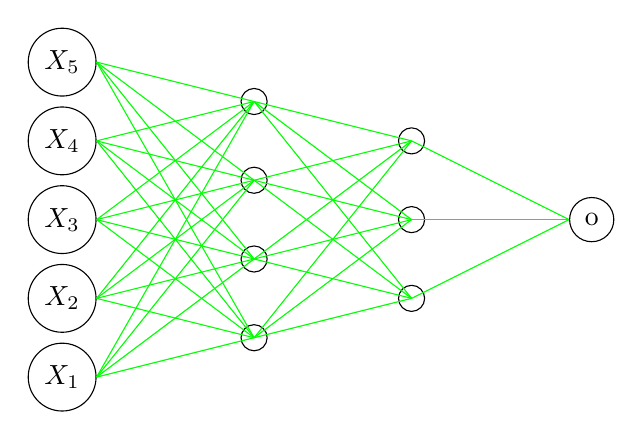
\begin{tikzpicture}
	\visible<2->{\foreach \y in {1,...,5} \draw(0,\y) node[left, circle, draw=black]{$X_\y$};
		\draw(6, 3) node[right, circle, draw=black]{o};}

	\visible<3->{\foreach \y in {1,...,4} \draw(2,\y+.5) node[circle, draw=black]{};
		\foreach \y in {2,...,4} \draw(4,\y) node[circle, draw=black]{};}
	\visible<4->{\foreach \y in {1,...,4} \foreach \i in {1,...,5} {\draw[green] (0,\i) -- (2,\y+.5);}
		\foreach \y in {2,...,4} \foreach \i in {1.5,...,4.5} {\draw[green] (2,\i) -- (4,\y);}
		\foreach \i in {2,...,4} {\draw[green] (4,\i) -- (6,3);}
	}
\end{tikzpicture}
\end{minipage}
\end{frame}

\begin{frame}

\frametitle{Restriction Bias}
\begin{itemize}
	\visible<2->{\item Restriction bias tells us what our model is able to represent}
	\visible<3->{\item Perceptron $\rightarrow$ can only split the data using a hyperplane}
	\visible<4->{\item Sigmoids $\rightarrow$ non-linear function}
	\visible<5->{\item What can we represent with a network?
		\begin{itemize}
			\visible<6->{\item Boolean Functions: Yes, because we have a network of threshold-like units}
			\visible<7->{\item Continuous Functions: Yes, with one (infinitely wide) layer}
			\visible<8->{\item Arbitrary Functions: Yes, with two (infinitely wide) layers}
		\end{itemize}
	}
	\visible<9->{\item{How do we make sure that we do not learn the arbitrary noise in the dataset, basically remembering it, but instead learn meaningful general rules?
			\begin{itemize}
				\visible<10->{\item Limit the number of neurons}
				\visible<11->{\item Dropout}
				\visible<12->{\item Weight Decay}
			\end{itemize}
		}
	}
\end{itemize}
\end{frame}

\begin{frame}
\frametitle{Optimizing Weights}
\begin{minipage}{.54\textwidth}
\begin{itemize}
	\item{There are multiple ways to use gradient descent.}
	\visible<2->{\item "Simple" Gradient Descent}
	\visible<3->{\item Advanced Methods
		\begin{itemize}
			\visible<4->{\item Momentum}
			\visible<5->{\item Higher Order Derivatives}
			\visible<6->{\item Randomized Optimization}
			\visible<7->{\item Penalty for Complexity}
		\end{itemize}
		
	}
\end{itemize}
\end{minipage}
\hfill
\begin{minipage}{.45\textwidth}
	\only<3->{\begin{tikzpicture}
		\begin{axis}[xlabel={$x$}, ylabel={$y$}, domain=0:1, width=\textwidth]
		\only<3->{\addplot+[no marks, domain=-1:1] {x*x*x*x-((x-.2)*(x-.2)};}
		\only<3->{
			\addplot+[scatter, only marks, scatter src=\thisrow{class},
			domain=0:1]
			table[x=x,y=y,col sep=comma,row sep=crcr] {
				x,y,class\\
				-.8,-.59,1\\
			};}
		
		\only<3->{
			\addplot+[scatter, only marks, scatter src=\thisrow{class},
			domain=0:1]
			table[x=x,y=y,col sep=comma,row sep=crcr] {
				x,y,class\\
				.9,.2,0\\
			};}
		\only<3->{
			\node[anchor=west] (source) at (axis cs:.89,.23){};
			\node (destination) at (axis cs:.5,-.3){};
			\draw[black, ->](source)--(destination);
			\addplot+[scatter, only marks, scatter src=\thisrow{class},
			domain=0:1]
			table[x=x,y=y,col sep=comma,row sep=crcr] {
				x,y,class\\
				.5,0,0\\
			};
			
		} 
		\end{axis}
		\end{tikzpicture}}
	
\end{minipage}

\end{frame}

\begin{frame}
\frametitle{Recurrent Neural Networks}
\begin{minipage}{.45\textwidth}
	\begin{itemize}
		\visible<2->{\item{Recurrent Neural Networks allow one to propagate states through time}}
		\visible<3->{\item{They calculate a hidden state $\vec{h_t}$ which is kept for the next time step, as $h_t = \sigma_h(W_hx_t + U_h h_{t-1} + b_h)$}}
		\visible<4->{\item{From this hidden state the current output is calculated as $y_t = \sigma_y(W_yh_t + b_y)$}}
		\visible<5->{\item{These networks cannot represent long-term dependencies as $U_h$ is always multiplied by itself.}}
	\end{itemize}
\end{minipage}
\hfill
\begin{minipage}{.54\textwidth}
	\begin{tikzpicture}
		\draw (0, 0) rectangle (1, 4);
		\foreach \y in {.5,...,3.5} \draw(.5,\y) node[circle, draw=black]{};
		\draw(-2, 1.5) node[left]{$\vec{x}$};
		\draw[->] (-2, 1.5) -- (0, 1.5);
		\draw[->] (1, 1.5) -- (3, 1.5);
		\draw[->] (1, 2.5) -- (2, 2.5) -- (2, 4.5) --node[above]{$\vec{h_t}$} (-1, 4.5) -- (-1, 2.5) -- (0, 2.5);
		\draw(3, 1.5) node[right]{$\vec{\hat{y}}$};
	\end{tikzpicture}
\end{minipage}

\end{frame}

\begin{frame}
\frametitle{LSTM}
\begin{minipage}{.49\textwidth}
\begin{itemize}
	\visible<2->{\item{LSTM (Long-Short-Term Memory) can store long term dependencies by adding a cell state and utilizing an input, forget and output gates.}}
	\visible<3->{\item{The input gate decides how much of the input and hidden states are stored to the cell state.}}
	\visible<4->{\item{The forget gate decides how much of the cell state shall be deleted.}}
	\visible<5->{\item{The output gate decides how much of the cell state is output to the hidden state.}}
\end{itemize}
\end{minipage}
\hfill
\begin{minipage}{.49\textwidth}
	
	\only<2->{
		\begin{figure}
			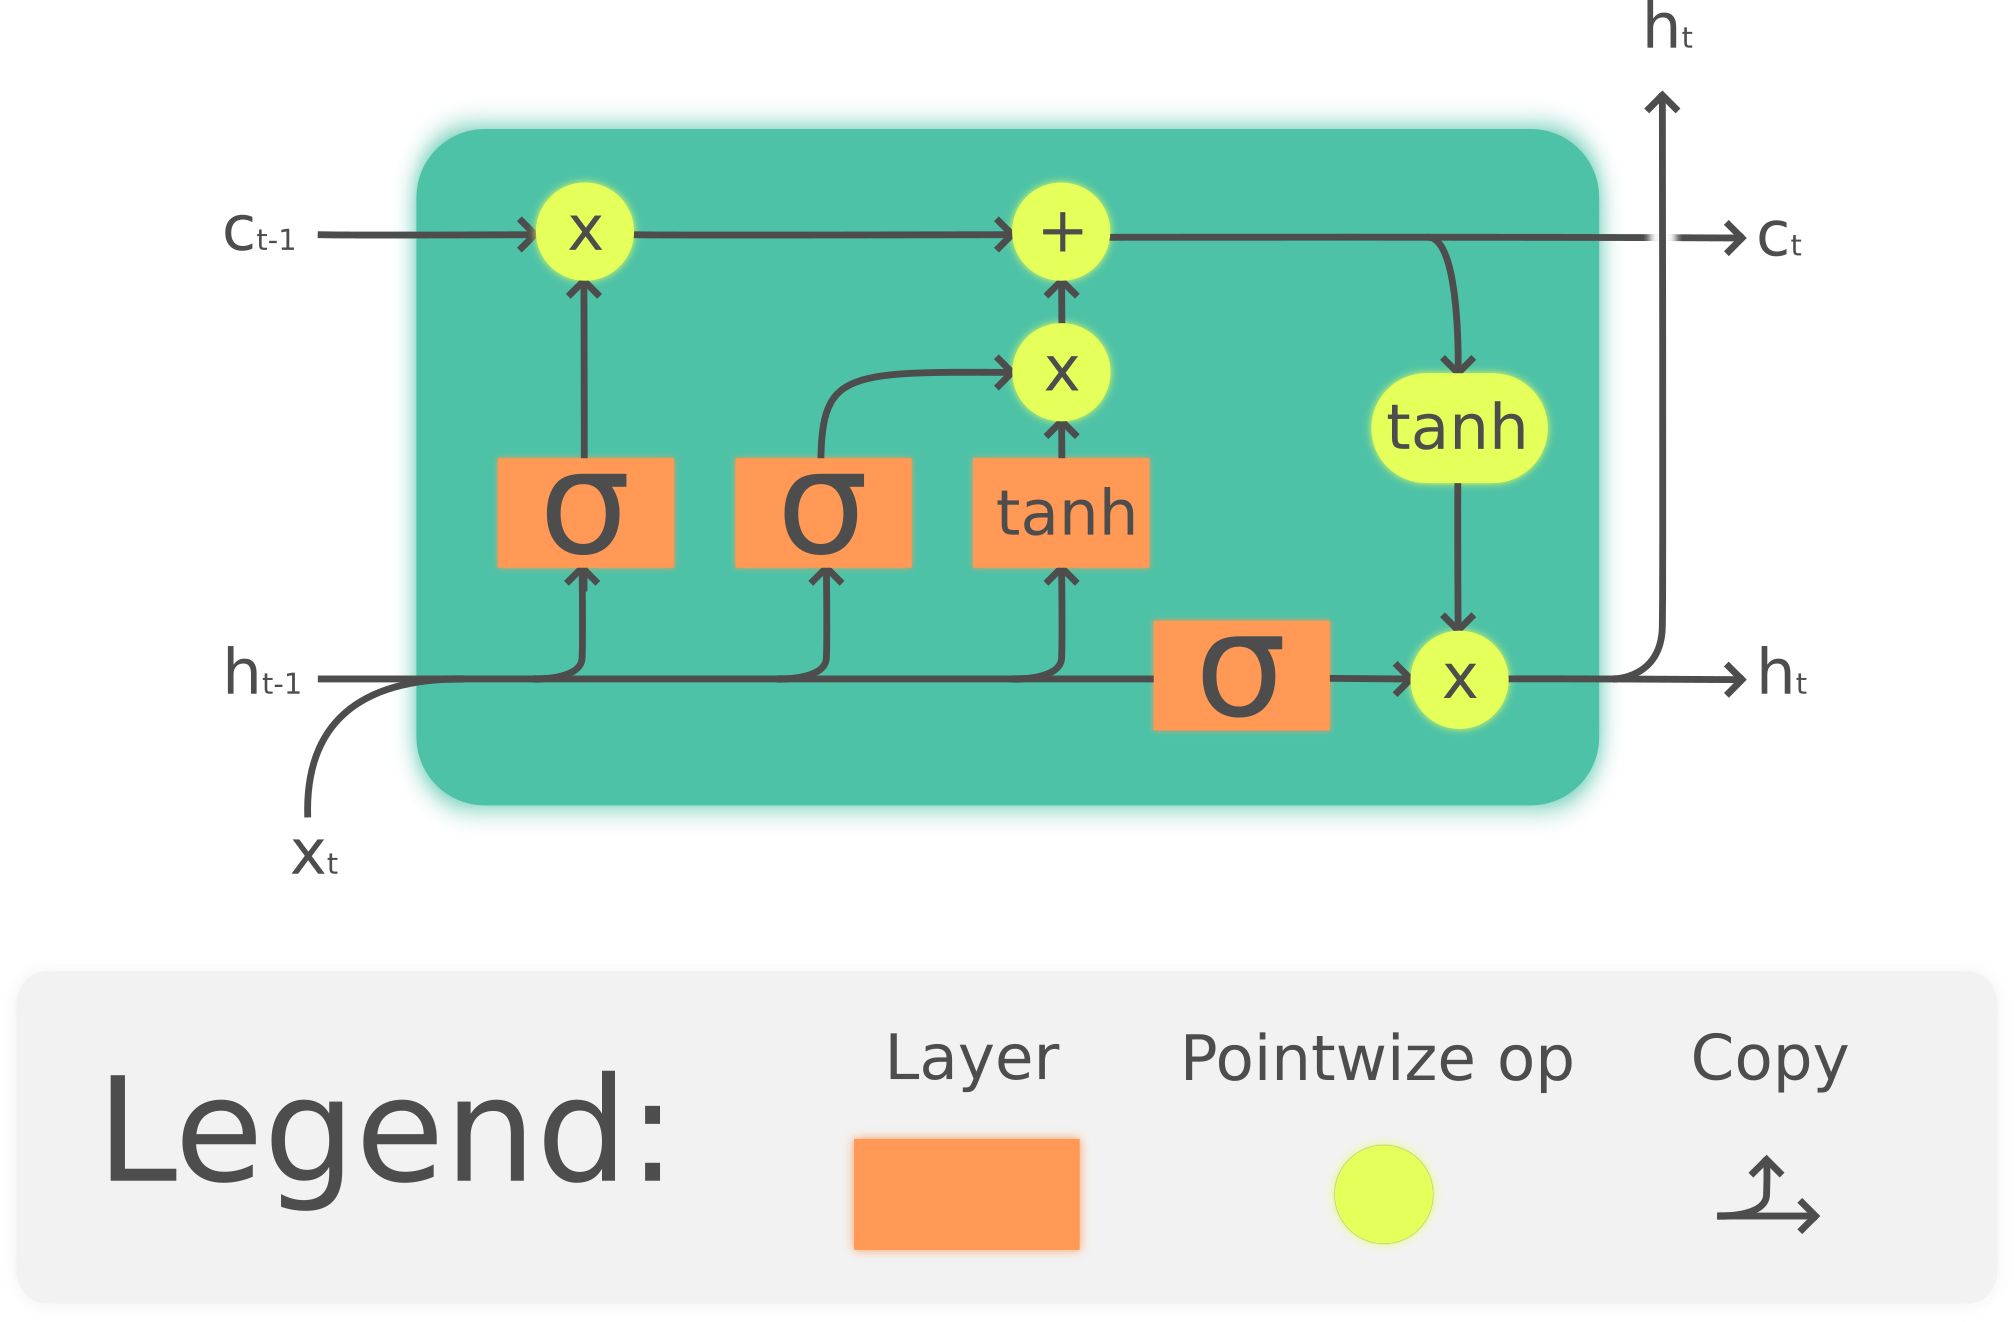
\includegraphics[width=\textwidth]{figs/The_LSTM_cell.png}
			\caption{Courtesy of \href{https://en.wikipedia.org/wiki/Long\_short-term\_memory\#/media/File:The\_LSTM\_cell.png}{wikipedia}}
		\end{figure}
		
	}
\end{minipage}
\end{frame}


\begin{frame}
\frametitle{Word2Vec}
\begin{minipage}{.49\textwidth}
	\begin{itemize}
		\visible<2->{\item{How can we turn text into numbers?}}
		\visible<3->{\item{Well let us use a neural network for this.}}
		\visible<4->{\item{Let us have a look at the sentence: "Pizza is awesome food". We can derive two tasks from it:
			\begin{itemize}
				\visible<5->{\item{Input "Pizza is \_\_\_\_ food" and let a network predict "awesome"}}
				\visible<6->{\item{Input "awesome" and let a network predict "Pizza", "is", and "food"}}
			\end{itemize}
		}}
		\visible<11->{\item{As classical training would update all the weights for each target example (where vocabularies can be million of words), the weights will only be updated for the right targets and a random selection of false targets}}
	\end{itemize}
\end{minipage}
\begin{minipage}{.49\textwidth}
	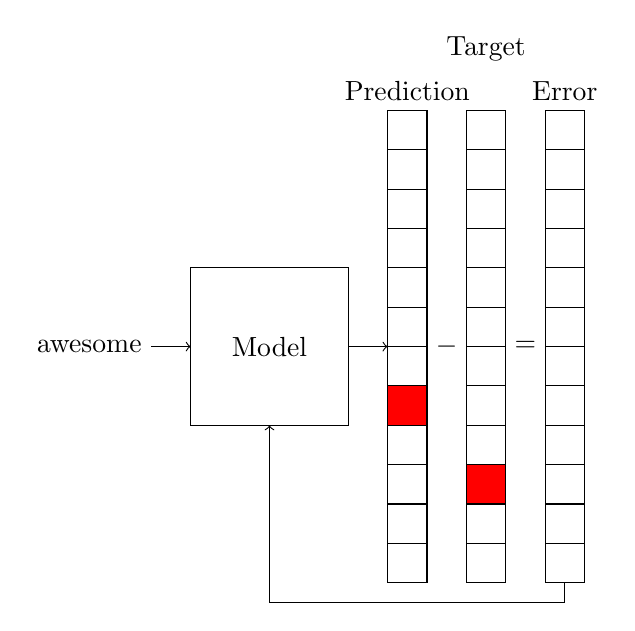
\begin{tikzpicture}\\
		\visible<7->{
			\draw (.5,0) coordinate (word) node[left]{awesome};
		
			\draw[->] (word) -- (1,0);
			\draw (1, -1) rectangle (3, 1);
			\draw (2, 0) node{Model};
			\draw[->] (3, 0) -- (3.5, 0);
			\draw (3.75, 3) node[above]{Prediction};
		
		
			\foreach \y in {-3, -2.5,...,2.5} \draw (3.5, \y) rectangle ++(.5,.5);
			\draw[fill=red] (3.5, -1) rectangle (4, -.5);
		}
	
		\visible<8->{
			\draw (4.75, 3.5) node[above]{Target};
			\foreach \y in {-3, -2.5,...,2.5} \draw (4.5, \y) rectangle ++(.5,.5);
			\draw[fill=red] (4.5, -2) rectangle (5, -1.5);
		}
		\visible<9->{
		
			\draw (4.25, 0) node{$-$};
			\draw (5.75, 3) node[above]{Error};
			\draw (5.25, 0) node{$=$};
			\foreach \y in {-3, -2.5,...,2.5} \draw (5.5, \y) rectangle ++(.5,.5);
		}
		\visible<10->{
			\draw[->] (5.75, -3) -- (5.75, -3.25) -- (2, -3.25) -- (2, -1);
		}
	\end{tikzpicture}
\end{minipage}

\end{frame}


\begin{frame}
\frametitle{Chatbot}
\begin{itemize}
\visible<2->{\item{Let's chat}}
\visible<3->{\item{The notebook we will use is inspired by the \href{https://pytorch.org/tutorials/beginner/chatbot_tutorial.html}{PyTorch chatbot tutorial}}, but it utilizes AllenNLP.}
\end{itemize}
\end{frame}

\begin{frame}
\frametitle{Encoder}
	\begin{minipage}{.49\textwidth}
		\begin{itemize}
			\visible<2->{\item To convert the words to vectors we will use \href{https://pytorch.org/docs/stable/nn.html?highlight=embedding\#torch.nn.Embedding}{nn.Embedding}. These can be trained as part of the neural network.}
			\visible<3->{\item We will then feed these vectors to a bi-directional encoder}
			\visible<4->{\item This will return output vectors for each time-step}
		\end{itemize}
	\end{minipage}
	\hfill
	\begin{minipage}{.49\textwidth}
		\visible<3->{
			\begin{figure}
				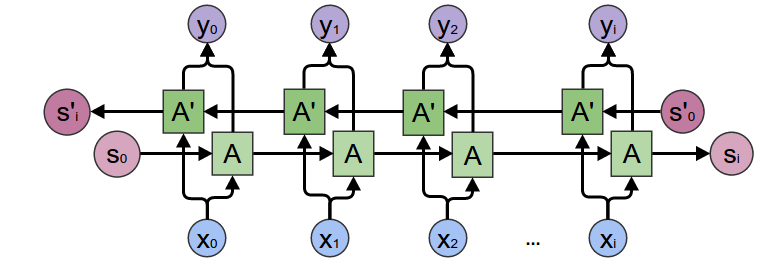
\includegraphics[width=\textwidth]{figs/BiEncoder.png}
				\caption{Image from \url{https://colah.github.io/posts/2015-09-NN-Types-FP/}}
			\end{figure}
		}
	\end{minipage}
\end{frame}

\begin{frame}
\frametitle{Attention}
\begin{minipage}{.49\textwidth}
\begin{itemize}
	\visible<2->{\item The decoder is build by a one directional recurrent neural network.}
	\visible<3->{\item The question is now how we input the vectors from the encoder to the decoder.}
	\visible<4->{\item We will let the neural network figure out what is important in each step using attention}
	\visible<5->{\item The attention mechanism will use the current output of the network and weight the encoder vectors accordingly}
	\visible<6->{\item It will then merge the weighted encoder vectors with the current decoder output}
\end{itemize}
\end{minipage}
\hfill
\begin{minipage}{.49\textwidth}
	\begin{figure}
		%\only<3-3>{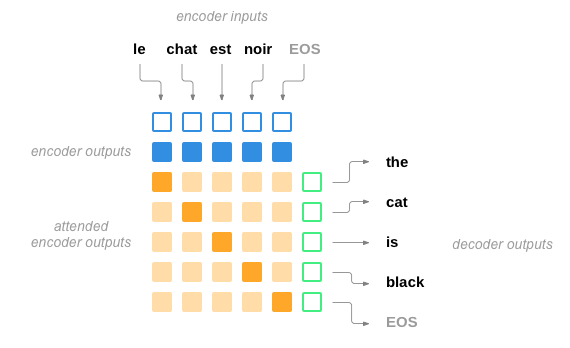
\includegraphics[width=\textwidth]{figs/attn1.png}}
		\only<4-5>{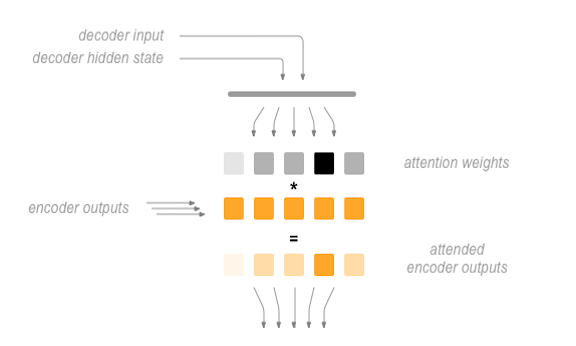
\includegraphics[width=\textwidth]{figs/attn2.png}}
		\only<4-5>{\caption{Courtesy of \href{  https://github.com/spro/practical-pytorch/blob/master/seq2seq-translation/seq2seq-translation.ipynb}{Sean Robertson}}}
		\only<6->{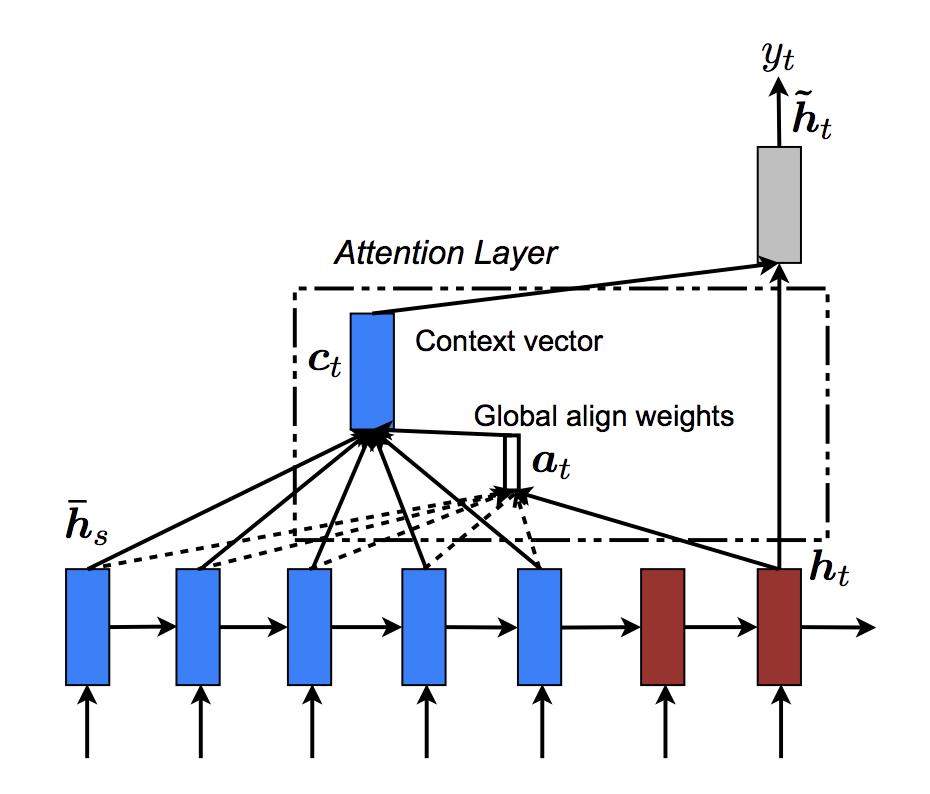
\includegraphics[width=\textwidth]{figs/global_attn.png}}
		\only<6->{\caption{From \href{  https://arxiv.org/pdf/1508.04025.pdf}{arxiv 1508.04025}}}
	\end{figure}

\end{minipage}
\end{frame}